% Grades of holdout 3 (run a) split by whether a relevant item reached the agent's context.
\begin{figure}[htbp]
\centering
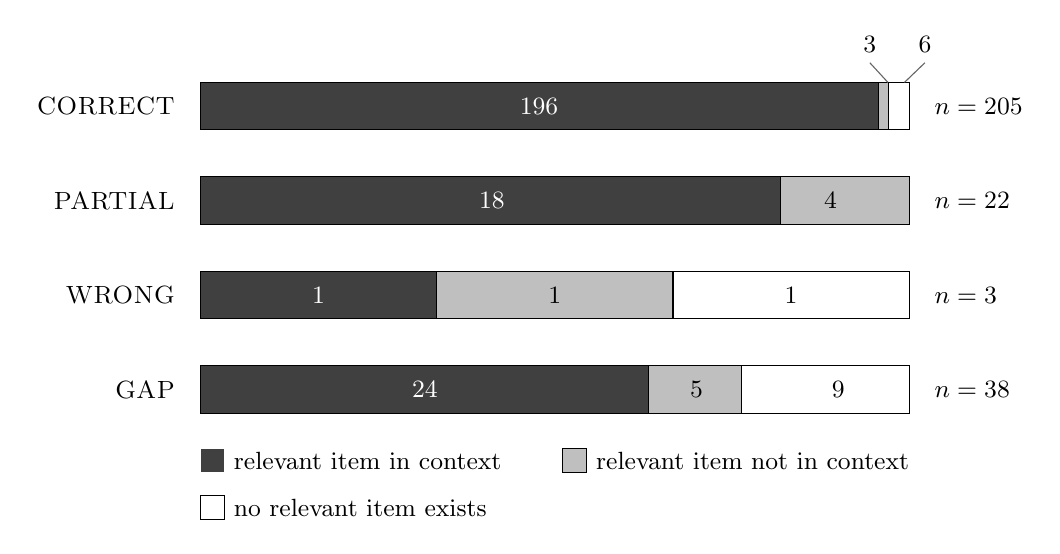
\begin{tikzpicture}[x=1cm,y=1cm,font=\small]
  \def\w{0.09}
  \fill[black!75] (0,-4.65) rectangle (0.3,-4.35);
  \node[right] at (0.3,-4.5) {relevant item in context};
  \fill[black!25,draw=black] (4.6,-4.65) rectangle (4.9,-4.35);
  \node[right] at (4.9,-4.5) {relevant item not in context};
  \fill[white,draw=black] (0,-5.25) rectangle (0.3,-4.95);
  \node[right] at (0.3,-5.1) {no relevant item exists};
  \foreach \y/\g/\a/\b/\c in {0/CORRECT/196/3/6, -1.2/PARTIAL/18/4/0, -2.4/WRONG/1/1/1, -3.6/GAP/24/5/9} {
    \pgfmathtruncatemacro{\n}{\a+\b+\c}
    \pgfmathsetmacro{\xa}{\a/\n*9}
    \pgfmathsetmacro{\xb}{(\a+\b)/\n*9}
    \node[left] at (-0.2,\y) {\textsc{\g}};
    \node[right] at ({100*\w+0.2},\y) {$n=\n$};
    \fill[black!75] (0,\y-0.3) rectangle (\xa,\y+0.3);
    \ifnum\b>0 \fill[black!25] (\xa,\y-0.3) rectangle (\xb,\y+0.3);\fi
    \ifnum\c>0 \fill[white] (\xb,\y-0.3) rectangle ({100*\w},\y+0.3);\fi
    \draw (0,\y-0.3) rectangle ({100*\w},\y+0.3);
    \ifnum\b>0 \draw (\xa,\y-0.3) -- (\xa,\y+0.3);\fi
    \ifnum\c>0 \draw (\xb,\y-0.3) -- (\xb,\y+0.3);\fi
  }
  % counts on the wide segments
  \node[text=white] at (4.3,0) {196};
  \node[text=white] at (3.7,-1.2) {18};
  \node at (8.0,-1.2) {4};
  \node[text=white] at (1.5,-2.4) {1};
  \node at (4.5,-2.4) {1};
  \node at (7.5,-2.4) {1};
  \node[text=white] at (2.85,-3.6) {24};
  \node at (6.3,-3.6) {5};
  \node at (8.1,-3.6) {9};
  % counts on the narrow segments of CORRECT
  \draw[black!60] (8.73,0.3) -- (8.5,0.55);
  \node[above] at (8.5,0.55) {3};
  \draw[black!60] (8.94,0.3) -- (9.2,0.55);
  \node[above] at (9.2,0.55) {6};
\end{tikzpicture}
\caption[Grades of holdout 3 (run $a$) by whether a relevant item reached the agent's context]{Grades of holdout 3 (run $a$) by whether a relevant item reached the agent's context. Each bar is scaled to 100 percent of the graded rows of its grade, and the numbers are row counts. \textsc{N/A} rows are omitted. Most answers that were not fully correct had a relevant item in context.}
\label{fig:error-attribution}
\end{figure}
